% !TEX root = ../main.tex
% Chapter Experiments results

\chapter{Results} % Main chapter title
\label{Chapter4} % Change X to a consecutive number; for referencing this chapter elsewhere, use \ref{ChapterX}

The main experiments' results are presented in this chapter. The different models trained are explicitely detailed in Appendix~\ref{AppendixB}.

\section{Data preprocessing}
Raw string sentence is preprocessed in order to give the encoder, and the decoder, a tokenized sequence. There are different steps to prepare data for training and these steps are illustrated in Figure~X. First, the raw sentence is tokenized to separate words and punctuation, the casing is not changed because it carries different information (e.g. start of sentence).

\begin{figure}
    \centering
    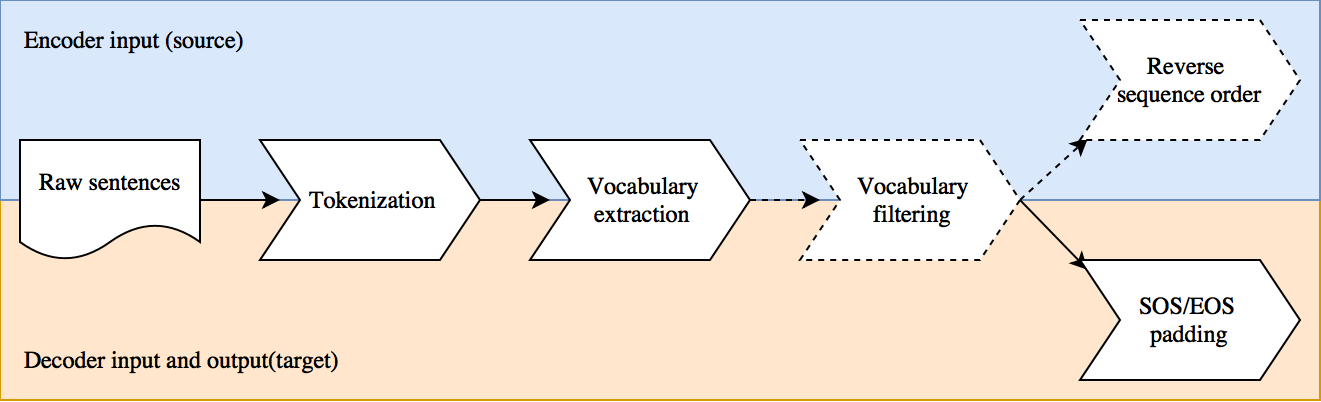
\includegraphics[width=\textwidth]{preprocess}
    \decoRule
    \caption[Preprocessing steps in NMT]{Preprocessing steps in an NMT model. Shapes with discontinued line refers to optional steps.}
    \label{fig:preprocess}
\end{figure}

Secondly, from the tokenized sentences, the preprocessor extracts the vocabulary (i.e. all the tokens with the number of times it appears). Table~\ref{tab:src-vocab} summarizes source vocabulary and Table~\ref{tab:tgt-vocab} summarizes target vocabulary.
Published work shows that people tend to limit the vocabulary. For example, \citet{1508.04025}, with a dataset of 4.5M sentence pairs (20 times the size of Cornell Movies Dialogs corpus), the vocabulary was limited to the 50K most frequent words. Additionnaly, in \citet{1506.06714}, with a dataset of 12M sentences, the vocabulary was also limited to the 50K most frequent words.
Table~\ref{tab:reduce-vocab} illustrates how both vocabularies can be reduced by using a threshold on word counts and only keep the most frequent ones.
In~\citet{1506.05869}, two different datasets were used. The first dataset contained 33M sentences and the vocabulary was limited to 20K words, and in the seconde dataset, composed of 88M sentences, the vocabulary was limited to 100K words.

\begin{table}
    \centering
    \caption[Source vocabulary analysis]{Source vocabulary analysis. Number of unique words:~64839}
    \label{tab:src-vocab}
    \begin{tabular}{ccc|c}
        \toprule
        \tabhead{Total count \%} & \tabhead{Unique words} & \tabhead{Vocabulary \%} & \tabhead{Current count value}\\
        \midrule
        90.0 & 1974 & 3.04 & 82\\
        97.0 & 12603 & 19.43 & 7\\
        98.0 & 19259 & 29.70 & 4\\
        99.0 & 32910 & 50.76 & 2\\
        99.9 & 61584 & 94.98 & 1\\
        \bottomrule
    \end{tabular}
\end{table}

\begin{table}
    \centering
    \caption[Target vocabulary analysis]{Target vocabulary analysis. Number of unique words:~65875}
    \label{tab:tgt-vocab}
    \begin{tabular}{ccc|c}
        \toprule
        \tabhead{Total count \%} & \tabhead{Unique words} & \tabhead{Vocabulary \%} & \tabhead{Current count value}\\
        \midrule
        90.0 & 1942 & 2.94 & 86\\
        97.0 & 12577 & 19.09 & 7\\
        98.0 & 19321 & 29.33 & 4\\
        99.0 & 33215 & 50.42 & 2\\
        99.9 & 62520 & 94.90 & 1\\
        \bottomrule
    \end{tabular}
\end{table}

\begin{table}
    \centering
    \caption[Vocabulary reduction]{Limiting the vocabulary size based on the word counts.}
    \label{tab:reduce-vocab}
    \begin{tabular}{ccc}
        \toprule
        \tabhead{Min count} & \tabhead{Vocabulary \%} & \tabhead{Total count \%}\\
        \midrule
        \multicolumn{3}{l}{\textit{Source vocabulary}}\\
        3 & 37.55 & 98.47\\
        5 & 25.38 & 97.66\\
        10 & 15.24 & 96.34\\
        \hline
        \multicolumn{3}{l}{\textit{Target vocabulary}}\\
        3 & 37.37 & 98.49\\
        5 & 25.39 & 97.69\\
        10 & 15.10 & 96.38\\
        \bottomrule
    \end{tabular}
\end{table}

The final step of the preprocessing is different from the source and target set. Source sentences can be reversed, word-wised, as mentionned to improve performance in \citet{1409.3215}.
Target sentences need to be padded with Start-Of-Sequence (SOS) and End-Of-Sequence (EOS) tokens to let the decoder know when the sequence starts and stops.

The source and target vocabularies present similar statistics because of the fact that most of the conversations present in the corpus have multiple turns. Thus, for example, conversation \code{[A, B, C, D]} is fed into the training set as \code{[(A,B), (B, C), (C, D)]} which makes \code{[B, C, D]} appear in both source and target sets.

\section{Runs}

There are four main runs that establish at the end the model parameters to create a chatbot based on the Cornell Movie Dialogs corpus. Among all the runs, except if specified, the dataset (i.e. training, development and test sets), model parameters specified in Table~\ref{tab:runs-shared-param} and the seed for model initialization are kept unchanged to avoid biases and measure effectively the different model parameters.

\begin{table}
    \centering
    \caption[Runs shared parameters]{Runs shared parameters.}
    \label{tab:runs-shared-param}
    \begin{tabular}{ll p{.5\textwidth}}
        \toprule
        \tabhead{Parameter} & \tabhead{Value} & \tabhead{Comment}\\
        \midrule
        \code{-{}-num\_train\_steps} & 12000 & Number of training steps\\
        \code{-{}-steps\_per\_stats} & 100 & - \\
        \code{-{}-random\_seed} & 27 & - \\
        \code{-{}-metrics} & bleu & BLEU score is used to evaluate the paramater text output\\
        \bottomrule
    \end{tabular}
\end{table}

The models' name follows a writing convention to allow the reader to instantly know the parameters used to train a particular model. All the names have the following form, the parameters are separated with a dash.
\begin{center}
    \codeg{run-20171212014119-norev-l8-u256-clstm-lr01-bw0-voc5}
\end{center}
The following list explains the different separated ``fields''.
\begin{itemize}
    \item \codeg{20171212014119}: which dataset the model was trained on
    \item \codeg{[no]rev}: if the input sequence is reversed or not
    \item \codeg{l8}: how many layers the model has, here 8
    \item \codeg{u256}: how many units the model has, here 256
    \item \codeg{clstm}: which RNN was used, here LSTM
    \item \codeg{lr01}: learning rate, here $0.1$
    \item \codeg{bw0}: beam width, here 0 so the decoding process uses gready search
    \item \codeg{voc5}: the count threshold used to filter out rare words from the vocabulary
\end{itemize}

\subsection{Run 1}
This run is focused on the neural network parameters. The exhaustive list of the parameters tested is illustrated in Table~\ref{tab:run01-params}. 72 models were trained by combining the parameters, on the whole vocabulary of the training set.

\begin{table}
    \centering
    \caption[Run 1 parameters]{Run 1 parameters measured.}
    \label{tab:run01-params}
    \begin{tabular}{ll p{.5\textwidth}}
        \toprule
        \tabhead{Parameter} & \tabhead{Values} & \tabhead{Comment}\\
        \midrule
        \code{-{}-num\_layers} & 2, 4, 8 & Network depth \\
        \code{-{}-num\_units} & 64, 128, 256 & Network size and emdeddings dimensionnality\\
        \code{-{}-cell} & lstm, gru & - \\
        \code{-{}-learning\_rate} & 1.0, 0.1 & - \\
        \code{-{}-beam\_width} & 0, 3 & If 0, decoding uses greedy search. If 3, decoding uses beam search\\
        \bottomrule
    \end{tabular}
\end{table}

Table~\ref{tab:run01-describe} shows the statistics for all the 72 models. The average time of training is about 70 minutes and the models presenting the minimum perplexities and maximum BLEU score are described in Table~\ref{tab:run01-best-models}.
\begin{table}
    \centering
    \caption[Run 1 performance stats]{Run 1 performance stats}
    \label{tab:run01-describe}
    \begin{tabular}{lrrrrr}
\toprule
{} &   \tabhead{dev\_bleu} &     \tabhead{dev\_ppl} &  \tabhead{test\_bleu} &    \tabhead{test\_ppl} &         \tabhead{Time [s]} \\
\midrule
mean  &   \num{0.023611} &  \num{270.738194} &   \num{0.009722} &  \num{234.481389} &  \num{4262.569444} \\
std   &   \num{0.072176} &  \num{166.934694} &   \num{0.041655} &  \num{153.184329} &  \num{1144.635582} \\
min   &   \num{0.000000} &   \num{86.710000} &   \num{0.000000} &   \num{67.680000} &  \num{2135.000000} \\
25\%   &   \num{0.000000} &  \num{107.485000} &   \num{0.000000} &   \num{85.395000} &  \num{3447.250000} \\
50\%   &   \num{0.000000} &  \num{172.050000} &   \num{0.000000} &  \num{142.400000} &  \num{4188.000000} \\
75\%   &   \num{0.000000} &  \num{458.630000} &   \num{0.000000} &  \num{406.577500} &  \num{5123.750000} \\
max   &   \num{0.400000} &  \num{462.410000} &   \num{0.200000} &  \num{409.810000} &  \num{6731.000000} \\
\bottomrule
\end{tabular}

\end{table}
\begin{table}
    \centering
    \caption[Run 1 best models]{Run 1 best models. The \textbf{maximum} value of the BLEU score and the \textbf{minimum} value of the perplexity are chosen.}
    \label{tab:run01-best-models}
    \begin{tabular}{lll}
        \toprule
        \tabhead{Metric} & \tabhead{Best} & \tabhead{Model}\\
        \midrule
        dev\_ppl & 86.71 & \code{run-20171212014119-norev-l2-u256-clstm-lr10-bw3-voca}\\
        dev\_bleu & 0.4 & \code{run-20171212014119-norev-l2-u64-cgru-lr01-bw0-voca}\\
        test\_ppl & 67.80 & run-20171212014119-norev-l2-u256-cgru-lr10-bw0-voca\\
        test\_bleu & 0.2 & run-20171212014119-norev-l2-u128-clstm-lr10-bw0-voca\\
        \bottomrule
    \end{tabular}
\end{table}

Since Table~\ref{tab:run01-best-models} shows four different models for the four metrics and no decision can be made on which paramaters trains the best model, Table~\ref{tab:run01-best-models-details} shows all the metrics for all the four models.

\begin{table}
    \centering
    \caption[Run 1 best models]{Run 1 best models with development and testing perplexity and BLEU score metrics.}
    \label{tab:run01-best-models-details}
    \begin{tabular}{llll}
        \toprule
        \tabhead{dev\_ppl} & \tabhead{dev\_bleu} & \tabhead{test\_ppl} & \tabhead{test\_bleu}\\
        \midrule
        \multicolumn{4}{l}{\textit{run-20171212014119-norev-l2-u256-clstm-lr10-bw3-voca}}\\
        86.71 & 0.00 & 68.89 & 0.00\\
        \hline

        \multicolumn{4}{l}{\textit{run-20171212014119-norev-l2-u64-cgru-lr01-bw0-voca}}\\
        172.04 & 0.40 & 141.75 & 0.20\\
        \hline

        \multicolumn{4}{l}{\textit{run-20171212014119-norev-l2-u256-cgru-lr10-bw0-voca}}\\
        86.73 & 0.10 & 67.68 & 0.00\\
        \hline

        \multicolumn{4}{l}{\textit{run-20171212014119-norev-l2-u128-clstm-lr10-bw0-voca}}\\
        94.54 & 0.10 & 75.34 & 0.20\\

        \bottomrule
    \end{tabular}
\end{table}

The question still to be answered is which parameter influences the most the performance of the model. Figures~XXX illustrates the models' test perplexity against the different parameters.

\begin{landscape}
\begin{figure}
    \centering
    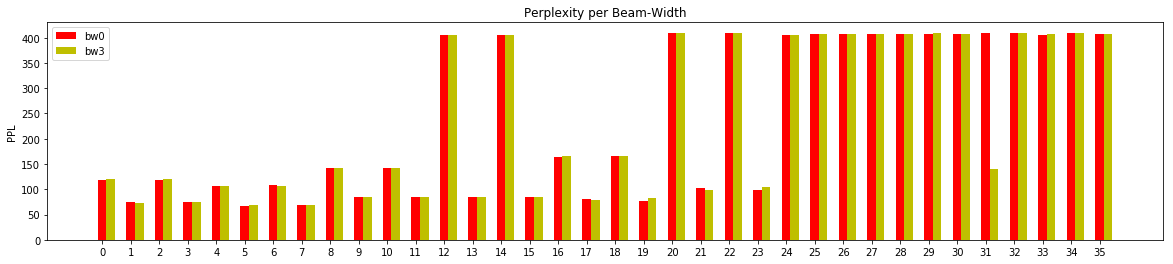
\includegraphics[width=\textheight]{res_run01_bw_ppl}
    \decoRule
    \caption[Results run01 BW-PPL]{Run01 results. Each color represents a beam-width value, x-axis represents the run number and y-axis the test perplexity.}
    \label{fig:res_run01_bw_ppl}
\end{figure}
\begin{figure}
    \centering
    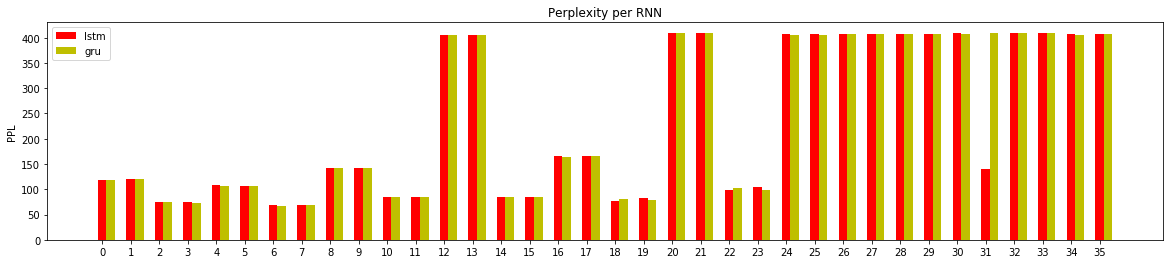
\includegraphics[width=\textheight]{res_run01_c_ppl}
    \decoRule
    \caption[Results run01 C-PPL]{Run01 results. Each color represents a RNN, x-axis represents the run number and y-axis the test perplexity.}
    \label{fig:res_run01_c_ppl}
\end{figure}
\begin{figure}
    \centering
    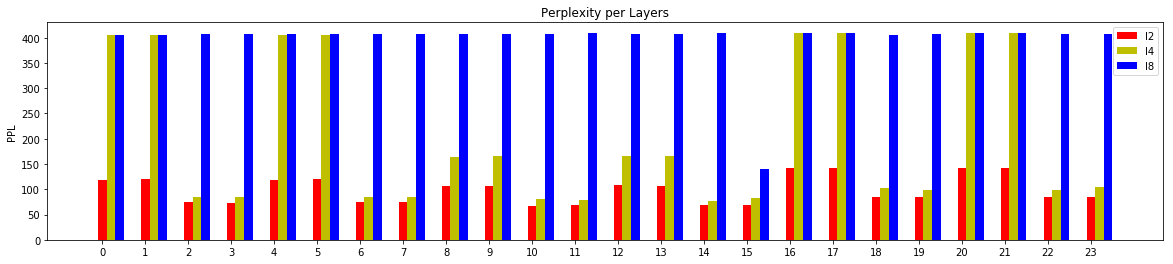
\includegraphics[width=\textheight]{res_run01_l_ppl}
    \decoRule
    \caption[Results run01 L-PPL]{Run01 results. Each color represents a layer value, x-axis represents the run number and y-axis the test perplexity.}
    \label{fig:res_run01_l_ppl}
\end{figure}
\begin{figure}
    \centering
    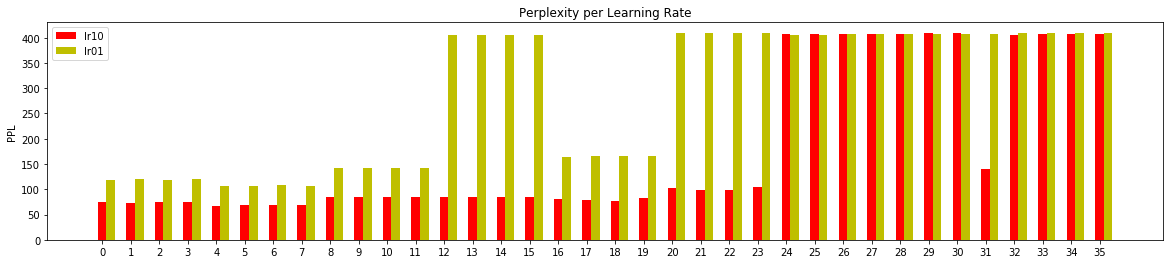
\includegraphics[width=\textheight]{res_run01_lr_ppl}
    \decoRule
    \caption[Results run01 LR-PPL]{Run01 results. Each color represents a learning rate value, x-axis represents the run number and y-axis the test perplexity.}
    \label{fig:res_run01_lr_ppl}
\end{figure}
\begin{figure}
    \centering
    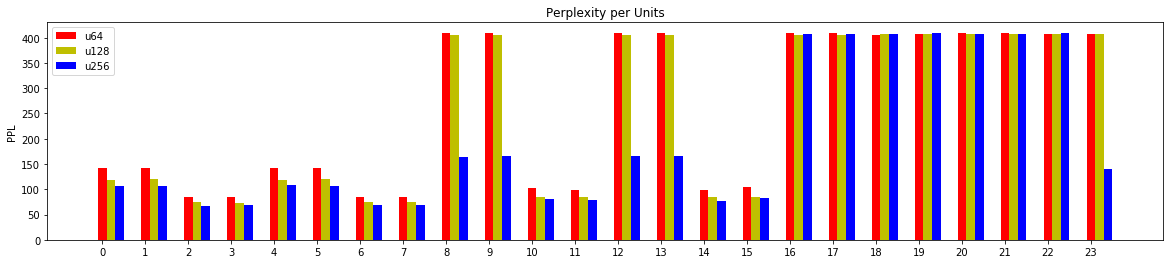
\includegraphics[width=\textheight]{res_run01_u_ppl}
    \decoRule
    \caption[Results run01 U-PPL]{Run01 results. Each color represents an unit value, x-axis represents the run number and y-axis the test perplexity.}
    \label{fig:res_run01_u_ppl}
\end{figure}
\end{landscape}

\subsection{Run 2}

\begin{landscape}
\begin{figure}
    \centering
    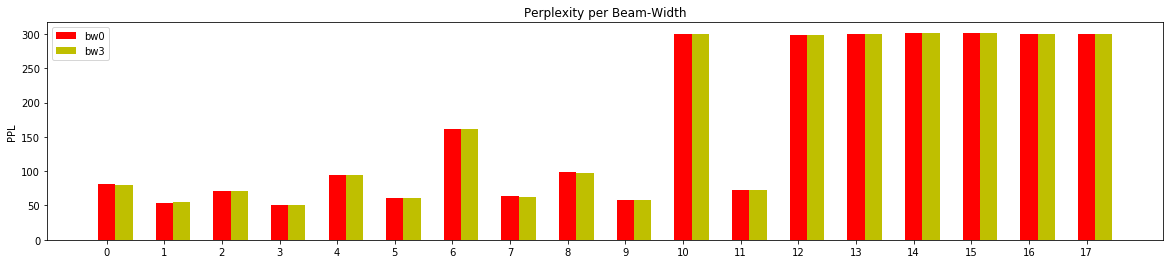
\includegraphics[width=\textheight]{res_run02_bw_ppl}
    \decoRule
    \caption[Results run02 BW-PPL]{Run02 results. Each color represents a beam-width value, x-axis represents the run number and y-axis the test perplexity.}
    \label{fig:res_run02_bw_ppl}
\end{figure}
\begin{figure}
    \centering
    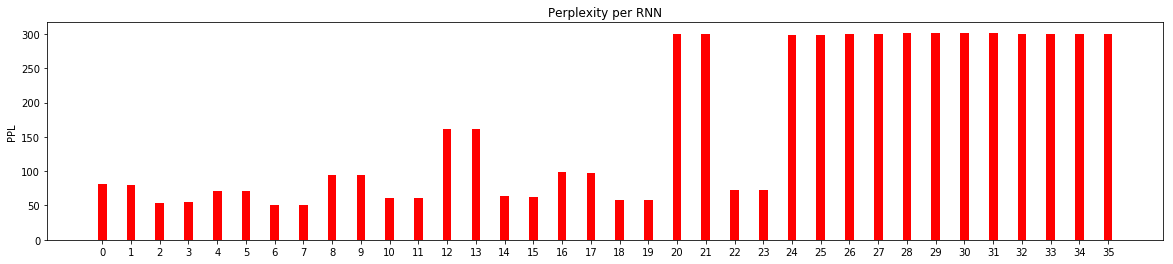
\includegraphics[width=\textheight]{res_run02_c_ppl}
    \decoRule
    \caption[Results run02 C-PPL]{Run02 results. Each color represents a RNN, x-axis represents the run number and y-axis the test perplexity.}
    \label{fig:res_run02_c_ppl}
\end{figure}
\begin{figure}
    \centering
    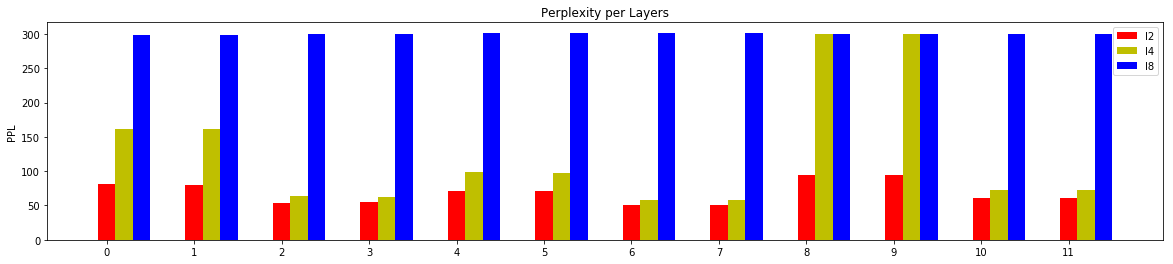
\includegraphics[width=\textheight]{res_run02_l_ppl}
    \decoRule
    \caption[Results run02 L-PPL]{Run02 results. Each color represents a layer value, x-axis represents the run number and y-axis the test perplexity.}
    \label{fig:res_run02_l_ppl}
\end{figure}
\begin{figure}
    \centering
    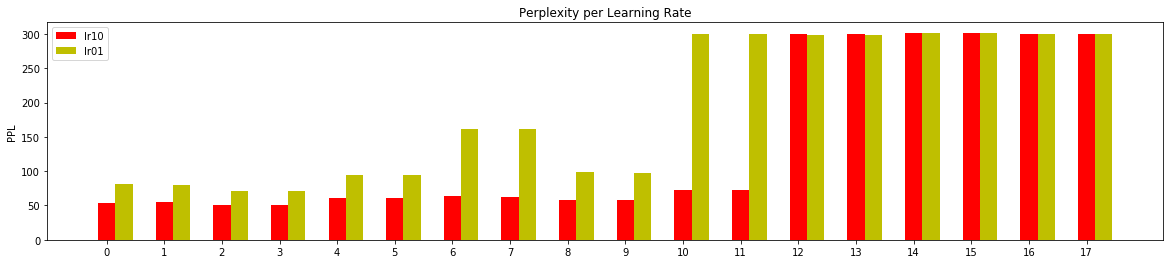
\includegraphics[width=\textheight]{res_run02_lr_ppl}
    \decoRule
    \caption[Results run02 LR-PPL]{Run02 results. Each color represents a learning rate value, x-axis represents the run number and y-axis the test perplexity.}
    \label{fig:res_run02_lr_ppl}
\end{figure}
\begin{figure}
    \centering
    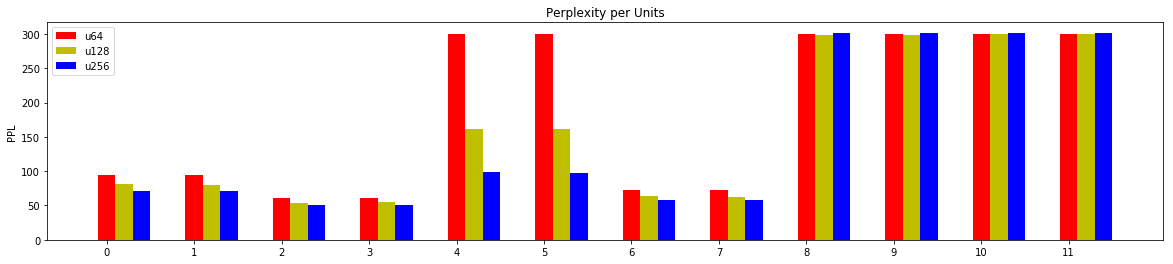
\includegraphics[width=\textheight]{res_run02_u_ppl}
    \decoRule
    \caption[Results run02 U-PPL]{Run02 results. Each color represents an unit value, x-axis represents the run number and y-axis the test perplexity.}
    \label{fig:res_run02_u_ppl}
\end{figure}
\end{landscape}

\subsection{Run 3}

\begin{landscape}
\begin{figure}
    \centering
    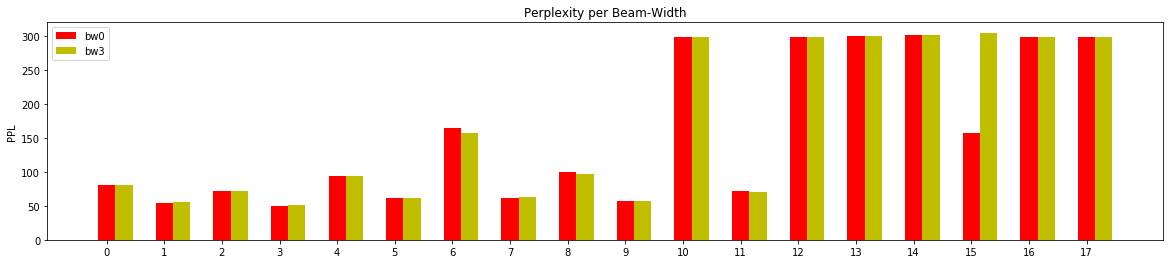
\includegraphics[width=\textheight]{res_run03_bw_ppl}
    \decoRule
    \caption[Results run03 BW-PPL]{Run03 results. Each color represents a beam-width value, x-axis represents the run number and y-axis the test perplexity.}
    \label{fig:res_run03_bw_ppl}
\end{figure}
\begin{figure}
    \centering
    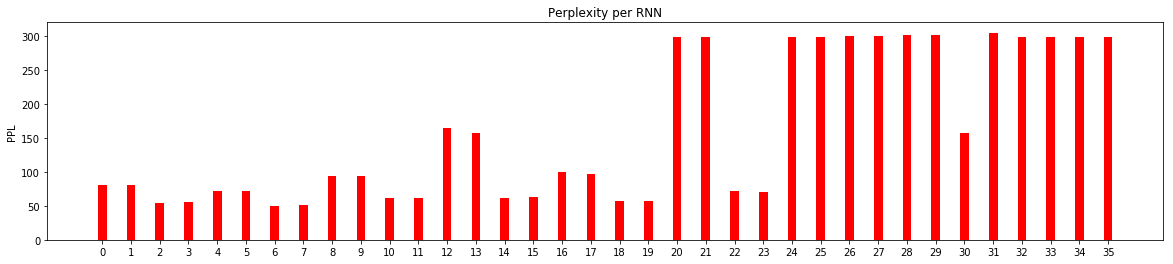
\includegraphics[width=\textheight]{res_run03_c_ppl}
    \decoRule
    \caption[Results run03 C-PPL]{Run03 results. Each color represents a RNN, x-axis represents the run number and y-axis the test perplexity.}
    \label{fig:res_run03_c_ppl}
\end{figure}
\begin{figure}
    \centering
    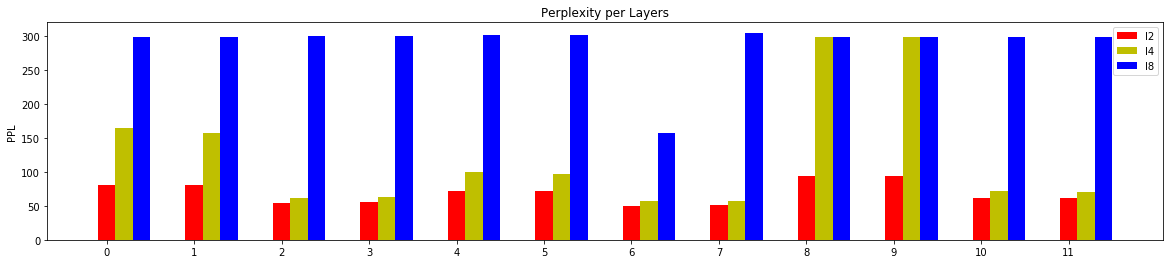
\includegraphics[width=\textheight]{res_run03_l_ppl}
    \decoRule
    \caption[Results run03 L-PPL]{Run03 results. Each color represents a layer value, x-axis represents the run number and y-axis the test perplexity.}
    \label{fig:res_run03_l_ppl}
\end{figure}
\begin{figure}
    \centering
    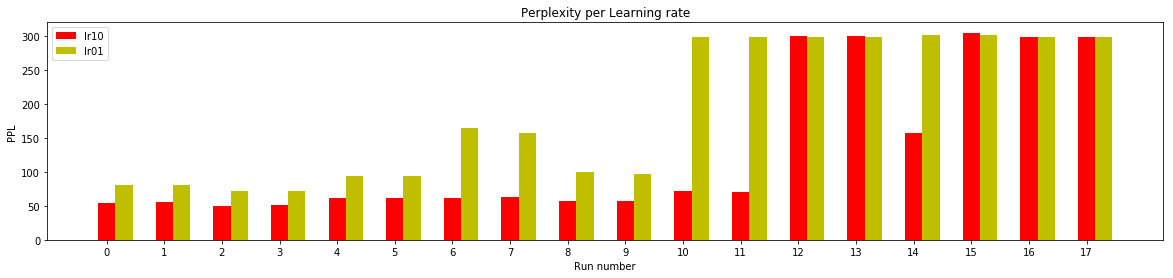
\includegraphics[width=\textheight]{res_run03_lr_ppl}
    \decoRule
    \caption[Results run03 LR-PPL]{Run03 results. Each color represents a learning rate value, x-axis represents the run number and y-axis the test perplexity.}
    \label{fig:res_run03_lr_ppl}
\end{figure}
\begin{figure}
    \centering
    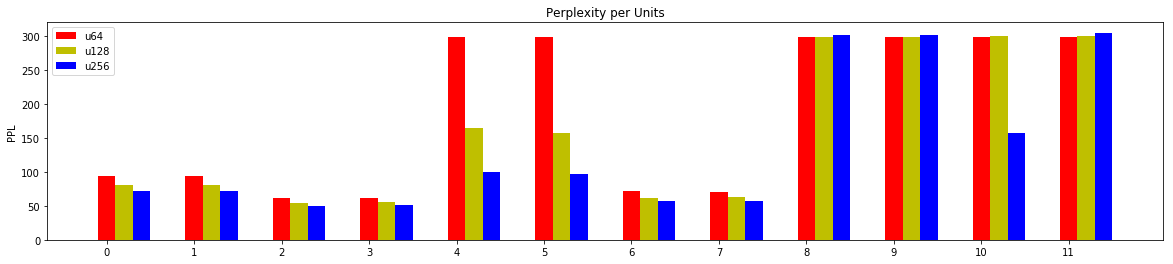
\includegraphics[width=\textheight]{res_run03_u_ppl}
    \decoRule
    \caption[Results run03 U-PPL]{Run03 results. Each color represents an unit value, x-axis represents the run number and y-axis the test perplexity.}
    \label{fig:res_run03_u_ppl}
\end{figure}
\end{landscape}

% Best parameters :
% LR 1.0
% BW 0 (greedy search best)
% C LSTM
% L 2
% U 512
% voc5
% rev
%
% Run todo:
% - at (luong / scaled_luong), bw (0 / 3), u (256 / 384 / 512) => 12 modeles
